\chapter{Array Synthesis}
So far we have discussed the problem of finding the radiation pattern given the array configuration and excitation which is called array analysis. However, this problem is not always the case in practice because most problems encountered in design are that the user specifies a radiation pattern and the designer is concerned with finding the array configuration and current excitation that would give the radiation pattern, and this problem is called the array synthesis problem. For instance, there may be an application where we would want to have a reception of some low-intensity signal but there is a strong interfering source located somewhere in a specific direction. We therefore would want to get the reception of the low-intensity signal and eliminate the radiation coming from the interfering source. The simplest way to do that is to place a null of the radiation pattern in the direction of the interfering source and then the radiation pattern appropriately (placing a null in the direction of the interfering source) then the low-intensity signal can be received effectively without modifying your receiving system. Other applications would rather want to illuminate a certain angular zone and then the power in the other direction would look like an angular sector. In practice, there are a variety of radiation patterns depending upon the application and now in this section, we would want to determine the array configuration and excitations which would give the flexibility of designing the radiation pattern.

The analysis of an array synthesis problem is not straight forward as an array analysis problem. We recall that there is no uniqueness in the solution for the current excitation given the radiation pattern and this makes the problem a difficult task. In this section, we will discuss the theoretical basis for synthesizing a radiation pattern and then consider some cases of radiation patterns such as radiation patterns specified by nulls or specified by illuminating zone.

\section{Schelkunoff Polynomial Method}
Consider an (N+1) element array equally spaced whose progressive phase shift is $\delta$ as shown in fig. \ref{fig:fig 55_1}. We would consider an observation point whose direction is $\phi$ with the axis of the array. The current excitation is non-uniform in amplitude and is in complex quantities. The reference current is $I_{N}$ given as $I_{N}=1\angle 0$
\begin{figure}[h]
\centering
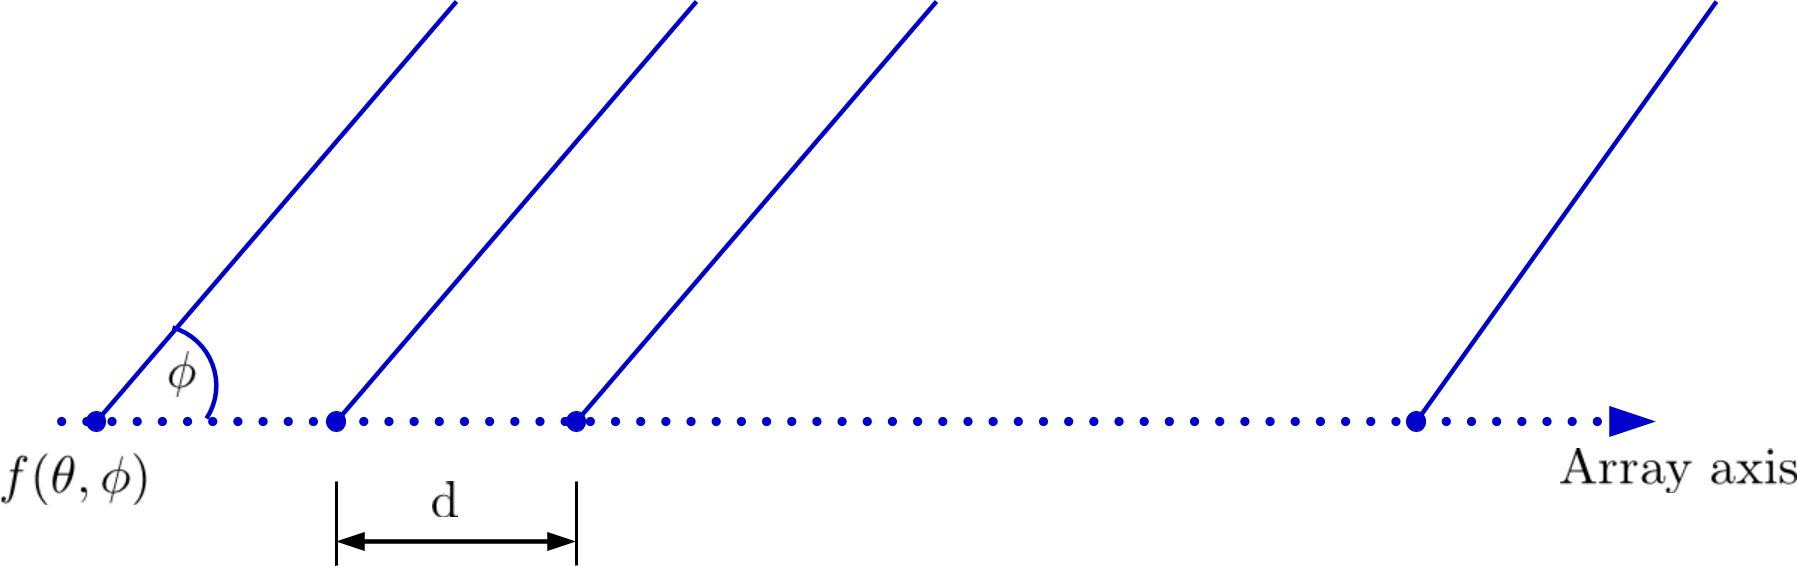
\includegraphics[width=1\linewidth]{/graphics/image58_1}
\caption{ General N-element, linear array}
\label{fig:fig 55_1}
\end{figure}

Just as before, the total electric field at the observation point is the superposition of all the electric fields of the antenna elements which is written as 
\begin{equation}
E_{T}=E_{o}\{I_{o}+I_{1}e^{j\psi}+I_{2}e^{j2\psi}+...+e^{jN\psi}\}
\label{eqn44}
\end{equation}
where $\psi$ is the phase of the array which is given as $\psi=\beta d\cos\phi$. It is apparent from Equation~\ref{eqn44} that the total electric field of the array is equal to the field of a single element (if the magnitude of the currents is the same) positioned at the reference multiplied by the factor which is widely referred to as the array factor. 

Thus Array factor,
\begin{equation}
AF=I_{o}+I_{1}e^{j\psi}+I_{2}e^{j2\psi}+...+e^{jN\psi}
\label{eqn45}
\end{equation}
 Let $$z=e^{j\psi}=x+jy$$, we can therefore rewrite Equation~\ref{eqn45} as
\begin{equation}
AF=I_{o}+I_{1}z+I_{2}z^{2}+...+z^N
\label{eqn46}
\end{equation}
which is a polynomial of degree N. From the mathematics of complex variables and algebra, any polynomial of degree N has N roots and can be expressed as the product of N linear terms. Thus we can write Equation~\ref{eqn46} as 
\begin{equation}
AF=(z-\zeta_1)(z-\zeta_2)(z-\zeta_3)+...+(z-\zeta_N)
\label{eqn47}
\end{equation}
where $\zeta_{1}$, $\zeta_{2}$, $\zeta_{3}$,...$z_{N}$ are the roots, which may be complex of the polynomial. The magnitude of Equation~\ref{eqn47} can be expressed as
\begin{equation}
|AF|=|(z-\zeta_1)(z-\zeta_2)(z-\zeta_3)...+(z-\zeta_N)|
\label{eqn48}
\end{equation}

A very important conclusion can be drawn from the above expression which is the roots of the polynomial corresponds to the nulls in the radiation pattern since the roots of a polynomial makes the polynomial zero.

The complex variable, we recall in 
$$z=e^j{\psi}=|z|\angle\psi = 1\angle\psi$$
where $$\psi=\beta d\cos\phi$$

It is clear that for any value of d or $\phi$, the magnitude of z lies always on a unit circle; however its phase depends upon d and $\phi$ suppose the solution of the polynomial given roots $\zeta_{1}$, $\zeta_{2}$, $\zeta_{3}$, $\zeta_{N}$ whose magnitude and phase varies. The magnitude of the roots which is unity (therefore lies on the unit circle) corresponds to the physical nulls as shown in fig.55- 2.
\begin{figure}[h]
\centering
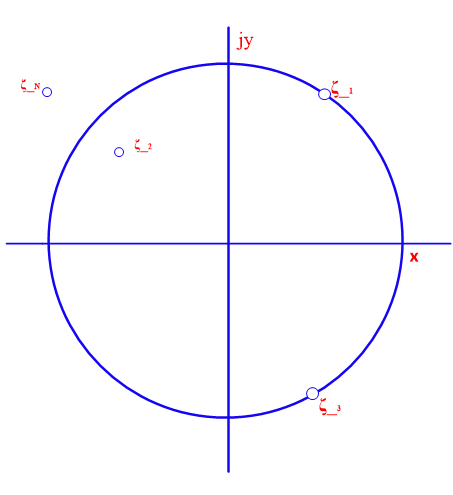
\includegraphics[width=1\linewidth]{/graphics/image58_2}
\caption{}
\label{fig:fig 55_2}
\end{figure}

We observe from fig.55-2 that the roots which lies on the unit circle are $\zeta_1$ and $\zeta_3$ and therefore the directions of the nulls can be gotten from $$z=e^{j\psi}=e^{j\beta d\cos\phi_{null}}=\zeta_1, \zeta_3$$ However the roots of the polynomial may not necessarily represent the null of the radiation pattern because for the root to represent the null it  must not only lie on the unit circle but also fall within the visible region of the polynomial space ($\phi=0$ to $\pi$).

We know $\psi=\beta d\cos\phi$ and for the visible range ($\cos\phi=+1$ to -1, $\psi=+\beta d$ to $-\beta d$) which depends on the values of d. So lets consider some cases for different values of d.\\
\textbf{Case I}: $\quad d=\dfrac{\lambda}{4}$
$$\beta d=\dfrac{2\pi}{\lambda}.\dfrac{\lambda}{4}=\dfrac{\pi}{2}$$ so the visible range of $\psi$ is $\dfrac{\pi}{2}$ to $-\dfrac{\pi}{2}$

Now let's plot the value of z, magnitude and phase as $\phi$ takes values from 0 to $\pi$ rad (called the circle diagram\footnote{\textcolor{blue}{The Circle diagram is the visualization of the roots of the polynomial on the complex z plane to see whether these nulls correspond to the physical nulls in the radiation pattern.}}).

It is observed that for $d=\dfrac{\lambda}{4}$ the values of z, for all physically observable angles of $\phi$, only exit over the part of the circle that lies in the visible range.
\begin{figure}[h]
\centering
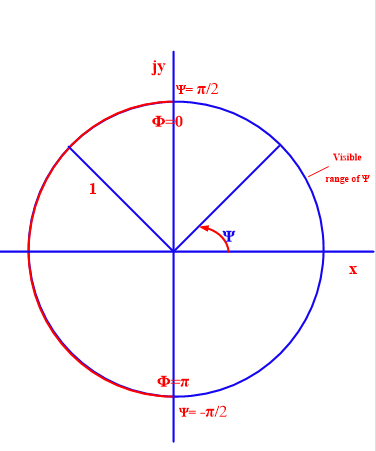
\includegraphics[width=1\linewidth]{/graphics/fig 55_3}
\caption{  Circle diagram for $d=\dfrac{\lambda}{4}$.}
\label{fig:fig-55-3}
\end{figure}

Any values of z outside the visible range are not realizable by any physical observation angle $\phi$ for the spacing $d=\dfrac{\lambda}{4}$.\\
\textbf{Case II}: $\quad d=\dfrac{\lambda}{2}$\\
We have, $$\beta d=\dfrac{2\pi}{\lambda}\cdot \frac{\lambda}{2} = \pi$$
so the visible range $\psi$ is $\pi$ to $-\pi$.

If we plot the range on the circle diagram as shown in fig. 55-4a, we get that the visible range of $\psi$ covers all the point on the circle. It is obvious that the visible range can be extended by increasing the spacing between the elements. So if we increase the value of d beyond $\dfrac{\lambda}{2}$ then the range of $\psi$ will overlap with itself.\\
\textbf{Case III}: $\quad d=\lambda$\\
We have, $$\beta d=\dfrac{2\pi}{\lambda}.\dfrac{\lambda}{2} = 2\pi$$
The visible range of $\psi$ is $2\pi$ to $-2\pi$. As we expect the range overlaps itself and it leads to multiple values for z. In this case we have double values for z for the full circle as shown in fig. 55-4b, which means we do not have an independent control of every point on the radiation pattern. That is as a certain point on the radiation pattern is defined.
\paragraph{}
We conclude then that the overall extent of a visible region can be controlled by the spacing between the elements and that the optimum choice of spacing is $d=\dfrac{\lambda}{2}$ because there is independent control and the entire range of $\psi$ is covered.
\begin{figure}[h]
\centering
\begin{minipage}[b]{0.4\textwidth}
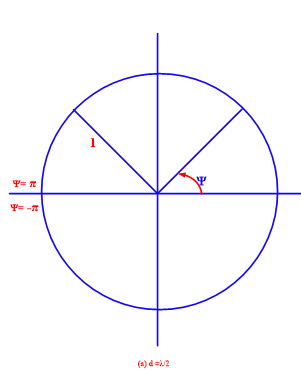
\includegraphics[width=1\linewidth]{/graphics/fig 55_4a}
\caption{Circle diagram for $d=\dfrac{\lambda}{2}$.}
\label{fig:fig-55_4a}
\end{minipage}
\hfill
\begin{minipage}[b]{0.4\textwidth}
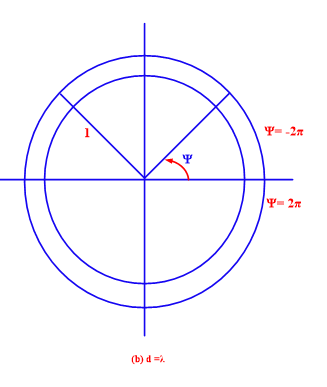
\includegraphics[width=1\linewidth]{/graphics/fig 55_4b}
\caption{Circle diagram for $d=\dfrac{\lambda}{2}$.}
\label{fig:fig-55_4a}
\end{minipage}
\end{figure}

\section{Array Specified by Nulls}
The circle diagram or Equation~\ref{eqn48} now can be used to synthesize an array which is completely specified by its nulls. The method used is the schelkunoff method and the procedure is as follows: 

\begin{enumerate}
\item[Step 1:] From the desired directions of nulls, $\phi_{n}$, find the corresponding $\psi_{n}$.
\item[Step 2:] Find the roots of the array polynomial, $\zeta
_n = e^{j\psi_{n}}$.
\item[Step 3:] Substitute $\zeta_n$ in the expression.
\begin{equation}
AF=|(z-\zeta_1)(z-\zeta_2)(z-\zeta_3)...+(z-\zeta_N)|
\label{eqn49}
\end{equation}
\item[Step 4:] Expand the polynomial in Equation~\ref{eqn49} in ascending powers of z.
\item[Step 5:] The coefficients of the polynomial are the complex excitation currents.
\end{enumerate}

Note that in this synthesis, one does not have any control over the direction of the main beam or the level of side-lobes etc. This type of synthesis is useful in an environment where there are many interfering sources in different directions and the array has to minimize the effect of interference on the signal.

\begin{exmp}
 Design a linear array with spacing between the elements  $d=\dfrac{\lambda}{2}$ such that it has nulls at $\phi=0$ and $\pi$rad. Determine the number of elements and the excitations. Use Schelkunoff's method.
\subsection*{\centering Solution}
Two nulls therefore means we need a minimum of 3 elements since $N=2$ so $(N+1)=3$ elements.
\begin{figure}[h]
 \centering
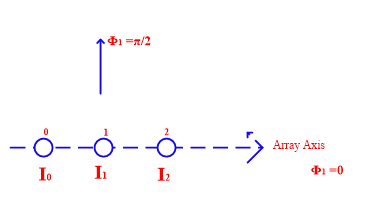
\includegraphics[width=1\linewidth]{/graphics/image58_3}
\caption{}
\label{fig:fig}
\end{figure}
\begin{enumerate}
\item[Step 1:] $$\psi_{1}=\beta d\cos\phi$$
 $$\beta=\dfrac{2\pi}{\lambda}$$ and $$d=\dfrac{\lambda}{2}$$
So $$\psi_{1}=\pi\cos\phi_{1}=\pi$$
and $$\psi_{2}=\pi\cos\phi_{2}=0$$
\begin{figure}[h]
\centering
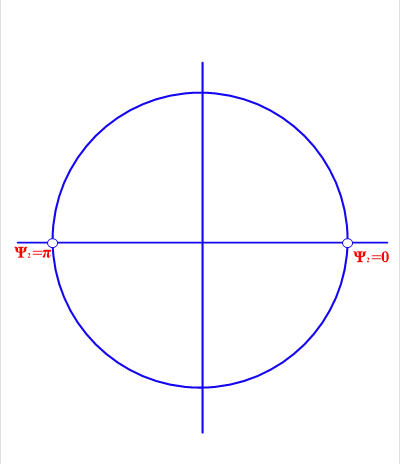
\includegraphics[width=1\linewidth]{/graphics/fig 55_5}
\caption{Circle diagram to specify the nulls.}
\label{fig:fig-55_5}
\end{figure}
\item[Step 2:] \begin{align*}
&\zeta_1 = e^{j\psi_{1}}=e^{j\pi}=-1\\
&\zeta_{2} = e^{j\psi_{2}}=e^{j0}=1
\end{align*}
\item[Step 3 and 4:]  \begin{align}
AF &=|(z-1)(z+1)|=|(z^{2}-1)|\nonumber\\
&=|-1+z^{2}|=|-1+0z^{1}+z^{2}|\nonumber	  
\end{align}	    	  
\item[Step 5:]  \begin{align*}
&I_{0}=-1=1\angle\pi\\
&I_{1}=0\\
&I_{2}=1=1\angle0
\end{align*}
\begin{figure}[h]
\centering
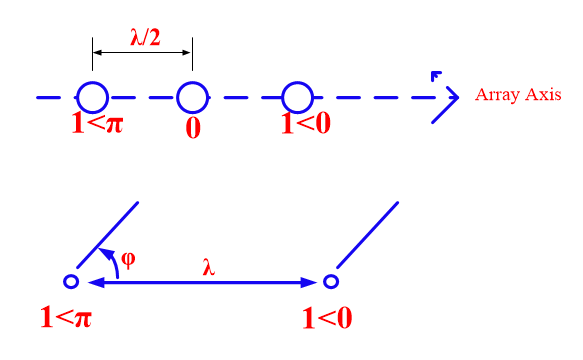
\includegraphics[width=1\linewidth]{/graphics/image58_4}
\label{fig:fig-55_6}
\end{figure}
\end{enumerate}
The radiation pattern can be gotten from the array factor assuming the antenna elements are isotropic. Thus

Radiation pattern, 
\begin{align*}
&F(\phi)=-1+z^{2}\\
&=-1+z^{2}\\
&=-1+e^{j2\pi\cos\phi} (z=e^{j\psi})\\
&=(-e^{-j\pi\cos\phi} + e^{j\pi\cos\phi} )e^{j\pi\cos\phi}\\
&=2j\sin(\pi\cos\phi)e^{j\pi\cos\phi}
\end{align*}
considering the magnitude of the radiation pattern $|F(\phi)|$ gives
\begin{equation}
|F(\phi)|= 2\sin(\pi\cos\phi)
\label{eqn50}
\end{equation}
From the equation, we get the corresponding nulls at $\phi = 0$ and at $\phi = \dfrac{\pi}{2}$, however, there is another null at $\phi =\pi$ which is due to the overlapping visible range in fig. \ref{fig:fig-55_5} (where $\psi = \pi$ and $\psi = -\pi$). This null is called the forced null and it can be avoided by reducing the visible region (shortening the physical angle $\phi$).
\end{exmp}
\begin{ExerciseList}
\Exercise[title=DIY]
\Question{Design a linear array with a minimum number of elements to have nulls at $\phi = 0, 45\deg$ and $120\deg$ where $\phi$ is the angle measured from the axis of the array. Choose inter- element spacing of $\dfrac{\lambda}{2}$.} 
\end{ExerciseList}
Answer: The array has four elements and the array excitation coefficients are (-0.7457 + j.6057), (1.4014 + j0.81), (1.6 + j0.2) and 1 